% Layout extracted from Kupzyk report at ca1d062; retain a descriptive title.
\documentclass[11pt]{article}
\usepackage[letterpaper,margin=0.82in]{geometry}
\usepackage{booktabs,longtable,array,graphicx,amsmath,xcolor,hyperref,xurl}
\usepackage[authoryear,round]{natbib}
\hypersetup{colorlinks=true,urlcolor=blue,linkcolor=blue,citecolor=blue}
\renewcommand{\arraystretch}{1.25}
\setlength{\emergencystretch}{1em}
\setlength{\parskip}{5pt}\setlength{\parindent}{0pt}
% Use scalable fonts; inspect pdffonts output after building. Avoid adding T1
% fontenc without an installed scalable font family. Add title/date in manuscript.

\newcommand{\Trials}{1920}
\newcommand{\MinRep}{20}
\newcommand{\MaxRep}{20}
\newcommand{\VarianceOutside}{191}
\newcommand{\PathOutside}{0}
\newcommand{\PositiveBands}{104}
\newcommand{\SourceAse}{0.04149}
\newcommand{\OursAse}{0.05907}
\newcommand{\PathAse}{0.04166}
\newcommand{\CostDays}{213}
\newcommand{\artifact}[1]{\href{https://github.com/alectionary/vibe-math/blob/master/formalization/schwabe-psychometric-genetics/#1}{\nolinkurl{#1}}}
\title{Measurement, missingness, and twin models:\\a whole-dissertation replication\\of Schwabe (2016)}
\date{30 October 2026}
\begin{document}
\maketitle
\begin{abstract}
We partly replicate Schwabe's dissertation-level results: published floor-effect slopes of 1.05 for sum scores and .03 for item analysis become 1.095 and $-.105$ in one full-length fit; the missing-covariate precision ordering agrees in all 108 primary point contrasts. Whole-dissertation replication remains incomplete: empirical inputs are unavailable and production simulation counts unfinished. The item-slope sign reversal is inconclusive, with posterior interval $[-.698,.439]$. MAR heritability overestimation is not established: at five covariates and 10\% missingness, the source gives .533 versus our .498 against truth .500; this opposite bias sign is also inconclusive. A published standard error of \SourceAse{} becomes \OursAse{} on the variance scale, versus \PathAse{} on the square-root path scale. The latter is an exploratory different-estimand reconstruction, not a reproduced procedure.
\end{abstract}

\begin{center}\small
\begin{tabular}{p{1.65in}p{1.25in}p{1.55in}p{.65in}p{.65in}}
\toprule Claim & Published & Ours & Same direction? & Verdict\\\midrule
Floor spurious interaction: sum minus item slope & $1.05-.03=1.02$ & $1.095-(-.105)=1.200$; one dataset & Yes & partial\\
Missing-covariate precision: deletion minus full SE & Positive point contrasts & Positive at all 108 primary cells & Yes & partial\\
MAR deletion heritability bias, $q=5$, 10\% missing & $.533-.500=+.033$ & $.498-.500=-.002$ & No; inconclusive & partial\\
Empirical interaction findings, Chapters 3--5 & Math $\beta_1=2.0837$; liberalism $-2.81$; SES $\beta_{1c}=-3.0777$ & No raw-data refits & Unknown & not established\\
Missing-data standard-error magnitude, one example & \SourceAse{} & \OursAse{} (variance); \PathAse{} (path) & Metric unresolved & partial\\
\bottomrule
\end{tabular}
\end{center}
\noindent\small The source values are from \citet[Tables 2.1, 3.2, 4.3, 5.4 and Figures 6.3 and 6.5]{schwabe2016}. Unavailable empirical fits are not established, not contradicted. Rounding agreement requires the same estimand to round half up to the printed value; the figure has no printed decimal precision. Conditional bands use our Monte Carlo error plus extraction bounds and do not recover source uncertainty. Positive deletion-minus-full SE means greater precision with full information.\normalsize

\section{What replicated, and what remains unestablished}
The measurement and missingness mechanisms receive partial support, while the dissertation's empirical conclusions remain unreplicated. The floor comparison gives a positive spurious sumscore slope and an item-level interval containing zero; the source's item-level point estimate is positive and ours negative, an inconclusive point reversal. The standard-error comparisons favor full information at every primary point contrast, but MAR heritability bias reverses point sign at five covariates and 10\% missingness: .533 in the source versus .498 here, against truth .500. Our adjusted bias interval includes zero, so the source overestimation finding is not established by this checkpoint. Neither result establishes the whole dissertation: original repeated-simulation summaries, several analytical assertions, and all empirical refits remain open.

The dissertation asks how measurement and incomplete covariates change genetic and environmental inference from twin data. It was awarded as a University of Twente PhD on 24 March 2016, supervised by C.A.W. Glas with adviser St\'ephanie M. van den Berg; the final published version has 154 numbered pages and 164 PDF pages. We read the full document, including all seven chapters and Appendices A--G. The 41-group inventory in Appendix~\ref{sec:coverage} treats every substantive original result as in scope. Cited background models and future extensions are distinguished from completed original work.

The central decomposition separates additive genetic variance $A$, shared environmental variance $C$, and individual environmental variance $E$. Monozygotic twins share genetic effects; dizygotic twins have genetic correlation one half. Item-response models connect latent phenotypes to observed item responses. Chapters 2--5 let environmental or genetic variance depend on a genotype or measured moderator; Chapter 6 models covariates jointly to retain incomplete observations.

\section{What we did ourselves, and what we took from others}
Our contribution is an auditable reconstruction and a full coverage inventory, not new empirical twin data. Schwabe supplied the models, designs, reported results and original programs. We wrote the simulation generators, fitting wrappers, source-vector extraction, comparisons, diagnostics and report. Original unlicensed programs and the full dissertation remain local; only limited attributed source crops are included. The Chapter 4 publisher supplement was checked separately \citep{schwabeConservatism}.

The statistical engines preserve the important model distinctions. R 4.5.0 \citep{r2025} runs JAGS 4.3.2 through rjags 4-16 for the Bayesian item-level models \citep{rjags2024}; coda 0.19-4.1 supplies posterior intervals and effective sample sizes \citep{coda2006}. OpenMx 2.21.13 fits the Chapter 6 Gaussian likelihoods \citep{neale2016}. lavaan 0.6-19 provides a second baseline ACE fit \citep{rosseel2012}. A covariance-only lavaan model would not reproduce the jointly moderated item likelihood, so that part explicitly uses the original JAGS engine family. The fitted likelihoods are implemented in \href{https://github.com/alectionary/vibe-math/blob/master/formalization/schwabe-psychometric-genetics/simulation/openmx_replication.R\#L15}{\nolinkurl{openmx_replication.R:15}} (joint model), \href{https://github.com/alectionary/vibe-math/blob/master/formalization/schwabe-psychometric-genetics/simulation/openmx_replication.R\#L31}{\nolinkurl{openmx_replication.R:31}} (conditional deletion model), and \href{https://github.com/alectionary/vibe-math/blob/master/formalization/schwabe-psychometric-genetics/simulation/jags_replication.R\#L24}{\nolinkurl{jags_replication.R:24}} (moderated item model).

The independent checks have limited independence. lavaan and OpenMx share one generated dataset and the ACE model; their baseline variance estimates differ by at most about $5\times10^{-8}$. SLSQP and CSOLNP share the Chapter 6 graph and data, checking optimization rather than model validity. Python's multivariate-normal generator checks R's conditional Gaussian generator through covariance moments. Original and reconstructed JAGS models share the engine and priors. Python 3.12.14 with \href{https://numpy.org/}{NumPy 2.3.5}, \href{https://scipy.org/}{SciPy 1.17.0}, \href{https://matplotlib.org/}{Matplotlib 3.10.8} and \href{https://pymupdf.readthedocs.io/}{PyMuPDF 1.26.6} supplies scalar checks, bands, plots and PDF inspection. R dependencies include \href{https://CRAN.R-project.org/package=MASS}{MASS 7.3-65} for Gaussian generation, \href{https://CRAN.R-project.org/package=matrixStats}{matrixStats 1.5.0} and \href{https://CRAN.R-project.org/package=foreign}{foreign 0.8-90} for package replay. These checks do not provide independent empirical evidence; \artifact{provenance/independence.json} states each boundary.

\section{Measurement effects: what the Bayesian attempts show}
The full-length floor example reproduces the qualitative contrast but not the published repeated-simulation estimates. At 500 pairs and 60 items, our sumscore slope is 1.095 with posterior standard deviation .181; the item-level slope is $-.105$ with posterior standard deviation .297. Both use the same generated response matrix. The repaired original centred JAGS program gives an item-level slope of $-.139$, compared with $-.105$ from the new non-centred representation. All five monitored posterior means fall inside exploratory five-comparison Monte Carlo bands; the largest point potential scale-reduction factor is 1.010, with upper bound 1.031. Effective sample sizes remain finite, so this is implementation agreement rather than proof of convergence or a repeated-simulation result (\artifact{outputs/posterior-comparison.csv}). The source reported averages over 100 datasets, 1.05 and .03, so these are not like-for-like Monte Carlo means. The difference is evidence to investigate, not a rounding discrepancy.

The four-chain convergence assessment uses rank-normalized folded split-$\widehat R$, bulk and tail effective sample sizes, and interval-endpoint diagnostics \citep{vehtari2021}, implemented with \href{https://github.com/stan-dev/posterior/tree/v1.6.1}{posterior 1.6.1}. Our operational criteria require $\widehat R<1.01$, bulk and tail effective sample sizes of at least 400, and mean Monte Carlo standard error no greater than 5\% of posterior standard deviation. Trace and rank plots and highest-posterior-density interval sensitivity remain separate checks; passing these numerical criteria does not prove convergence.

The ceiling and symmetric sumscore fits supply supporting directional checks. Our ceiling slope is $-.857$, versus the reported $-1.08$; the symmetric case is .100, versus the reported mean .03 and between-replication standard deviation .24. Our posterior standard deviations are not substitutes for that between-replication standard deviation. Full results, intervals, effective sample sizes and chain lengths are in \artifact{outputs/confirmation-c2-floor.csv}, \artifact{outputs/confirmation-c2-floor-sums.csv}, \artifact{outputs/confirmation-c2-ceiling-sums.csv}, and \artifact{outputs/confirmation-c2-symmetric-sums.csv}.

Every published Bayesian simulation arm was attempted, and most remain unresolved. The twelve sample-size/effect cells of Tables 2.2--2.3 and all seven sample-size/item-count cells of Tables 5.1--5.2 have actual full-size-data pilot fits. Their short chains cannot establish power, parameter recovery, or convergence. The original curvilinear experiment on page 26 lacks a recoverable design and numerical results. Its absence is retained as a blocker, not converted to an excluded result. The source numerical targets are in \artifact{outputs/source-simulation-targets.csv} and \artifact{outputs/source-power-targets.csv}.

The production cost is substantial, rather than a reason to redefine the dissertation. At 8,000 pairs, a separate timing run used ten burn-in and ten retained iterations; the measured sampling cost projects to about \CostDays{} single-worker elapsed days for that condition's 250 source-length repetitions alone. This is a rough extrapolation, not a hard execution denial or a completed attempt at those repetitions. Initialization, adaptation, parallel scaling and mixing can change it. The production target remains open in \artifact{outputs/resource-projection.json}.

\section{Missing covariates: direction and numerical scale}
Full information reduces the estimated variance-component standard errors in all 108 primary point contrasts at this checkpoint. The complete grid includes three missingness mechanisms, four covariate counts and three stated missingness proportions; a fourth, 3\%, tests the conflicting plot labels. There are \Trials{} method-by-dataset fits, with \MinRep{} repetitions per condition at the recorded checkpoint. The original used 1,000 per condition. The primary contrast is $\mathrm{SE}_{\mathrm{deletion}}-\mathrm{SE}_{\mathrm{full}}$; its sign is separate from an ours-minus-source reproduction deviation.

The mean contrast is simultaneously positive in \PositiveBands{} of the 108 primary comparisons under the stated approximation. We use paired differences across independently generated datasets, save two-standard-error intervals, and apply Bonferroni-adjusted Student intervals across the 108 primary contrasts \citep{dunn1961}; the 36 extra 3\% contrasts form a separate family. Small-sample normal-mean approximations and selection of assumptions after the initial pilots limit these bands. They are not equivalence tests. The complete records are \artifact{outputs/signed-contrasts.csv} and \artifact{provenance/uncertainty-plan.json}.

The plotted magnitudes remain unresolved on the printed variance scale. For example, with two covariates and low MCAR missingness, the source's additive-genetic standard error is approximately \SourceAse{}, whereas ours is \OursAse{}. Across the 216 source SE values, \VarianceOutside{} lie outside conditional adjusted bands for variance SEs. Those bands include our Monte Carlo error and a conservative quarter-PDF-point extraction bound, but omit unknown source Monte Carlo error; they cannot establish an author error or a complete two-sample disagreement.

An exploratory change of metric explains much of the difference. For a positive path $a$ with variance $V=a^2$, the delta-method relation is $\mathrm{SE}(V)=2|a|\mathrm{SE}(a)$. Reconstructing path SEs gives \PathAse{} in the example, and \PathOutside{} of the 216 path-scale comparisons lie outside the corresponding conditional bands. These are different estimands. Agreement with a transformed expression does not prove that it was the source procedure; the original plotting and standard-error extraction code would settle that question. The printed variance-scale comparison is preserved in \artifact{outputs/source-comparisons.csv}.

The extraction retains every source curve, not just the illustrative example. We read vector paths for Figures 6.3--6.6, calibrated their axes against tick labels, and checked rendered evidence. The CSV retains coordinates, drawing identifiers and extraction bounds: \artifact{outputs/source-figure-values.csv}. Source point orderings have unknown uncertainty. The table below concerns standard-error ordering only. The bias inventory is separate.
{\small\begin{longtable}{p{2in}p{1.8in}p{2.5in}}
\toprule
Condition & Source / ours contrast & Interpretation\\\midrule\endhead
All conditions & No point reversal & Both metrics and low-missingness readings retained in \artifact{outputs/signed-contrasts.csv}.\\
\bottomrule\end{longtable}}

Figure 6.5's bias findings require a separate signed contrast: estimate minus generating truth, with positive meaning overestimation. All 72 MAR method/parameter/condition cells are in \artifact{outputs/bias-contrasts.csv}. There are 23 source-versus-ours point-sign reversals; 19 source signs exceed the extraction bound. None of these reversals has our Bonferroni-adjusted 72-comparison interval excluding zero. For deletion heritability at five covariates and 10\% missingness, source .533154 and ours .497505 lie on opposite sides of truth .5. Our bias $-.002495$ has adjusted interval $[-.098004,.093014]$. This is an inconclusive point reversal, not evidence of an opposite established bias. The family was added during independent review and is exploratory; source Monte Carlo uncertainty remains unknown. \artifact{simulation/bias_contrasts.py} retains two-SE and adjusted intervals, extraction bounds and separate ours-minus-source deviations.

\section{Assumptions}
\subsection{Regression coefficients and covariate means}
The stated explained variance fixes a quadratic form, not the individual coefficients. We use equal positive coefficients satisfying $\beta^\mathsf{T}(\Sigma_W+\Sigma_B)\beta=.64$, yielding total variance 1.64 and explained fraction .39024. A distinct unequal-coefficient sensitivity retains the same explained variance. The main reconstruction estimates a mean for each covariate; the Appendix F script ties them together. We test the shared-mean restriction separately. Neither supplied choice establishes the missing original driver.

\subsection{Low missingness and moderator allocation}
The thesis gives 2\% in the Chapter 6 design and captions but 3\% in plots and parts of the discussion. Both are retained; neither is silently selected because it agrees better. For Chapter 5 we assume a balanced binary moderator, consistent with a .7 main effect explaining approximately 11\% of variance. The exact moderator allocation and random seeds were not recovered. The alternative sample-size reading of 80,000 in the prose is not a completed arm: Table 5.1 and its discussion specify 8,000, which is the implemented primary reading.

\subsection{Priors, initialization, and historical software}
The reconstructed Bayesian priors follow the source precision/variance conventions. The current and pre-defense BayesTwin repositories were both tested; an exact source-era session specification remains unavailable. New random seeds and a non-centred parameterization are explicit departures from unavailable original drivers. They must not be used to claim identical stochastic output. The full-length original-program comparison tests the same posterior on the same generated input, while source-length repeated grids remain open.

\section{Ambiguities that were resolved locally}
\subsection{Program identifiers and modern R conditions}
Appendix A fails with its documented inputs because it references \texttt{ndz}, \texttt{n.items} and \texttt{Ydz} instead of the documented names. Repairing only those identifiers allows sampling. Appendices B, D and E compile without those repairs, and Appendix G samples after local PDF whitespace/page-label normalization. These are executable checks, not empirical validation: \artifact{outputs/original-programs.csv} and \artifact{outputs/appendix-g-result.txt}.

The current BayesTwin code encounters a vector-condition error under R 4.5.0. Applying an explicit scalar test to the initialization check permits all twelve model/item-family smoke tests to return. The pre-defense revision has separate failures, including inconsistent-category initialization and a missing ADE prior argument. These are recorded alongside successes in \artifact{outputs/bayestwin-checks.csv} and \artifact{outputs/historical-bayestwin.csv}; the later package \citep{bayestwin} is not substituted silently for the 2016 source.

\subsection{Printed probability and information expressions}
Two literal printed expressions do not match the implemented models under simple checks. At zero trait and thresholds with unit discrimination, Equations 4.6--4.9 give probabilities summing to 1.25; the Appendix B cumulative-softmax program gives probabilities summing to one. For Equation 3.4, a discrimination of two at response probability one half gives printed information .25, while finite-difference score information is 1.00. The usual discrimination-squared factor explains this difference. We checked the rendered expressions in \artifact{evidence/eq4-probabilities.png} and \artifact{evidence/eq3-information.png}. Neither check establishes that the empirical fitted programs or Figure 3.2 used those literal expressions.

\subsection{Identification versus likelihood uniqueness}
The logvariance coefficients are uniquely determined by known component variances at two distinct moderator values, but this does not establish a unique likelihood maximum. Write the conditional phenotype variance as $V=A+C+E$, with twin covariances $K_{\mathrm{MZ}}=A+C$ and $K_{\mathrm{DZ}}=A/2+C$. Then $A=2(K_{\mathrm{MZ}}-K_{\mathrm{DZ}})$, $C=2K_{\mathrm{DZ}}-K_{\mathrm{MZ}}$, and $E=V-K_{\mathrm{MZ}}$. For a positive component variance $v(m)=\exp(\beta_0+\beta_1m)$, its values at $m_0\ne m_1$ determine $\beta_1=[\log v(m_1)-\log v(m_0)]/(m_1-m_0)$ and then $\beta_0$. These are conditional algebraic results: they assume the latent covariance functions are known. They do not prove that those functions can be identified from the observed item responses.

The extra squared-path ambiguity depends on moderator support. For a shared binary moderator, replacing the slope $b$ by $-2a-b$ in $(a+bm)^2$ preserves the variances at $m=0,1$. The example paths $(a,b)=(.5,.2)$ and $(.5,-1.2)$ therefore agree at those endpoints but differ at $m=.5$, where their variances are .36 and .01. If two squared affine paths agree at three distinct moderator values, their difference is a polynomial of degree at most two with three roots, hence identically zero. Factoring that polynomial shows that only a global sign change remains; a positive-intercept convention removes it. This qualifies the extension of the binary argument to continuous moderators in \citet[Appendix C, pp.\ 138--139]{schwabe2016}; it does not establish full marginal item-model identification.

A valid finite dataset also shows why an injective variance parameterization cannot guarantee a finite likelihood maximum. Suppose every observed Rasch response is zero. Holding the remaining finite parameters fixed, write each latent trait as $\mu+Z$. The conditional probability of the observations is a finite product of terms $\operatorname{logit}^{-1}(b_k-\mu-Z)$, each strictly increasing as $\mu$ decreases. Its expectation therefore increases strictly and tends to one as $\mu\to-\infty$, by dominated convergence, while remaining below one at every finite $\mu$. Thus no finite likelihood maximizer exists for this dataset. This counterexample qualifies the unrestricted uniqueness statement on page 72; it does not show multiple maxima for the dissertation's samples or an improper Bayesian posterior. A proper prior changes the posterior objective. The written arguments, assumptions, exact symbolic checks and numerical illustration are recorded in \artifact{provenance/identification-check.json} and \artifact{simulation/identification_check.py}; \artifact{evidence/p72-identification-claim.png} shows the source wording.

\subsection{Identification from calibrated item responses}
A reviewed conditional argument identifies the Chapter 5 calibrated Gaussian item model from its observed response distribution, including known unequal positive item discriminations. It requires two distinct item observations that are conditionally independent given the trait, known finite calibration, positive latent variances, and both MZ and DZ groups represented at each of two moderator levels. The source reports positive OPLM discriminations \citep[p.\ 40]{schwabe2016}, but the empirical calibration, observation process and joint support were not independently verified from raw data. This is a population-identification argument; it does not establish finite-sample likelihood uniqueness or successful empirical estimation.

One marginal item probability and a within-person joint probability identify latent mean and variance. Let $f(t)=L(a_1t-d_1)$ and $g(t)=L(a_2t-d_2)$, with known $a_1\geq a_2>0$, finite $d_1,d_2$, logistic $L$, and trait $\mu+sZ$ for standard-normal $Z$ and $s>0$. For each $s$, fixing $p=E[f(\mu+sZ)]$ determines a unique $\mu$. Along that curve, the derivative of $q=E[f(\mu+sZ)g(\mu+sZ)]$ is $E[f']\operatorname{Cov}_w(Z,r)$, where $w$ weights the normal density by $f'$ and $r=(fg)'/f'$. Writing $c=a_2/a_1$, direct differentiation gives
\[
 r=g+c\frac{g(1-g)}{1-f},\qquad
 r'=a_2g(1-g)\frac{1+c(1-2g)}{1-f}>0.
\]
The numerator bracket is $(1-c)+2c(1-g)>0$, so the covariance is strictly positive. Although $r$ may be unbounded, $f'r=(fg)'$ is bounded, which supplies the weighted integrability needed here. Thus $q$ increases strictly with $s$ at fixed $p$, determining $s$ and then $\mu$. Identical calibrations are allowed, but reusing the same response twice would violate the required conditional independence.

With mean and variance determined, a cross-twin joint item probability increases strictly with Gaussian latent covariance $K$: differentiating the density and integrating by parts gives $dE[f_j(\mu+X)f_k(\mu+Y)]/dK=E[f_j'(\mu+X)f_k'(\mu+Y)]>0$. MZ and DZ joint probabilities therefore determine their covariances; the ACE inversion and two-level formulas recover the mean and logvariance coefficients. The complete regularity and support conditions are in \artifact{provenance/joint-item-identification-check.json}, with independent mathematical review in \artifact{provenance/joint-item-identification-independent-review.json}. This is a reviewed written argument with symbolic checks, not a Lean-certified result. Its formalization gap remains separate from its mathematical review.

\subsection{Illustrative curves and simulated point clouds}
The two item-characteristic curves in Figure 1.3 can be reconstructed geometrically with equal logistic discrimination approximately two and difficulties approximately $-2$ and $-.5$ on the printed axes. The maximum vertical residual is .00725 PDF points. An independent linearization of the logit agrees with the nonlinear fit; a unit-discrimination curve on the same axes misses by about 18--21 points. These are reconstructed figure coordinates, not recovered original generating parameters. The caption states equal discrimination, and a latent-scale rescaling changes its numerical value. This check therefore supports the illustrated ordering without establishing a source error or the original plotting procedure.

Figure 7.1 contains 10,000 markers in each panel and supports the intended contrast between nearly perfect and moderate genetic--phenotypic association. Reconstructed sample correlations are .99950 and .70955, respectively. The first panel's reconstructed residual sample variance is approximately .0010, but a conservative quarter-point geometric uncertainty envelope includes zero; it cannot establish a nonzero population residual variance. The source labels an approximate illustration, and its seed and driver remain unavailable. Independent marker-center and axis-calibration checks are retained in \artifact{provenance/illustration-followup.json}, \artifact{provenance/illustration-independent-review.json}, and \artifact{simulation/illustration_followup.py}. These are source-figure reconstructions, distinct from our newly generated illustrative samples.

\section{Empirical results and summary reconstructions}
The original empirical conclusions cannot be refitted from the obtained materials. Chapter 3 requires NTR responses and Cito calibration; Chapter 4 requires Virginia30K responses; Chapter 5 additionally requires linked SES; Chapter 6 requires linked school and twin records. All twelve public author repositories were cloned and audited before these gaps were declared. The available BayesTwin example is explicitly simulated output, not a substitute empirical dataset.

Published-mean calculations provide limited checks with a different scope. The Chapter 3 one-standard-deviation environmental ratios reconstruct as 1.6316 and 1.8489, rounding to 1.63 and 1.85. A ratio of the printed variance means gives heritability .7292, whereas the reported posterior mean is .7286; these need not be equal because expectation and nonlinear division do not commute. The same distinction applies to Chapter 4. The sign reversals between its item and sumscore analyses are source-reported findings, not fresh empirical replications.

The illustrative figures can be partly regenerated without raw data. We simulated 10,000 MZ pairs from the Chapter 3 printed mean parameters, reconstructed conditional variance curves, and generated both Chapter 7 genetic/phenotypic illustrations. Original posterior bands and score histograms remain blocked. See \artifact{outputs/ch3-mz-illustration.pdf}, \artifact{outputs/conditional-variance.pdf} and \artifact{outputs/ch7-illustration.pdf}.
{\small\begin{longtable}{p{1.7in}p{.8in}p{.8in}p{.75in}p{.8in}p{1in}}
\toprule
Claim & Published & Ours & Precision & Numerical & Scope\\\midrule\endhead
Ch6 MCAR,q2,low missing; A variance SE & 0.04149 & 0.05907 & Figure-derived & Not judged & Limited\\
Same condition, path SE & Metric not stated & 0.04166 & Figure-derived & Not comparable & Limited\\
Ch2 floor beta1: sum / IRT & 1.05 / .03 & 1.095 / -.105 & .01 in source & Not comparable & Limited; one dataset\\
Ch2 ceiling beta1, sums & -1.08 & -.857 & .01 in source & Not comparable & Limited; one dataset\\
Ch2 symmetric beta1, sums & .03 & .100 & .01 in source & Not comparable & Limited; one dataset\\
Ch3 AxE one-SD ratio & 1.63 & 1.6316 & .01 & match & Limited\\
Ch3 AxC one-SD ratio & 1.85 & 1.8489 & .01 & match & Limited\\
Ch3--6 empirical fitted results & Original tables & Not estimated & Table-specific & No verdict & Unavailable\\
\bottomrule\end{longtable}}
The first two rows separate a labelled variance SE from an exploratory path SE; neither inherits a decimal tolerance from a figure-derived display. The next three rows compare a single dataset with a source Monte Carlo average and therefore have no numerical verdict. The ratio rows use the source formula and round to the printed values, but retain limited scope. Empirical fits have unavailable scope. Per-family comparability records are in \artifact{provenance/comparability.json}.

\section{What remains unresolved}
The largest remaining causes differ by result, and the stopping statements preserve that distinction. For empirical claims, missing raw responses, calibration and linkage inputs rank ahead of software choices; repository and supplement searches did not recover them. For Bayesian simulation summaries, insufficient repeated converged fits rank ahead of numerical discrepancies; all cells were piloted, source-length cases and original-program checks were attempted, and actual resource costs were measured. The exact curvilinear design remains unavailable.

For the Chapter 6 magnitude gap, the standard-error estimand currently ranks ahead of optimizer differences. We checked vector extraction against the ink, retained variance versus path metrics, compared SLSQP with CSOLNP, checked covariance algebra independently, and ran unequal-coefficient and shared-mean sensitivities. These checks do not recover the original random seeds, beta allocation, session versions or plotting driver. The most informative single artifact would be the original Chapter 6 simulation-and-summary script. No author contact was made.

Independent scientific review identified missing bias contrasts and continuation bookkeeping defects; these have been corrected while preserving the original numerical baseline. Independent rendered-manuscript review checks the final PDF, source hashes and evidence in \artifact{provenance/review.json}. This review does not establish successful whole-dissertation replication. Completion of execution attempts is also distinct from successful replication. None of the open production or empirical items is closed as outside a selected scope.

\section{Code and source availability}
The dated availability audit below is part of the evidence, not a claim that every possible repository was exhaustively searched. Institutional metadata and the author-hosted source identify the edition; source hashes and repository revisions are in \artifact{provenance/source.json} and \artifact{provenance/author-repositories.json}. Full copyrighted source files remain local. The following rows copy \artifact{provenance/availability.json}.
{\small\begin{longtable}{p{1.8in}p{4.6in}}
\toprule
Place/date & Result\\\midrule\endhead
Institutional final-version record / 2026-10-30 & Verified PhD, institution, advisers, date, DOI, ISBN and final-version designation.\\
Author dissertation GitHub repository / 2026-10-30 & Full164-page thesis and five model programs obtained at6c2c48901209fc76ba932bb094c61abba5ef160d. No raw empirical datasets or Monte Carlo driver/seeds. Full text read. Original files kept local; rights reserved/no code license.\\
All12 public author GitHub repositories / 2026-10-30 & All cloned; immutable hashes in \artifact{provenance/author-repositories.json}. Data-file and code audit found workshop data, BayesTwin simulated posterior example and unrelated projects; no matching NTR/Cito/Virginia study inputs or curvilinear simulation driver. This is a search limit, not proof of absence.\\
OSF indexed search / 2026-10-30 & Queries site:osf.io Schwabe twin and exact Inga Schwabe2016 found later unrelated projects/preprints, no matching dissertation simulation or empirical input. No identified thesis OSF project.\\
GitLab indexed search / 2026-10-30 & Queries Schwabe and exact ingaschwabe returned unrelated authors/no matching repository. No claim of exhaustive private-site search.\\
Zenodo indexed search / 2026-10-30 & Queries Schwabe twin and exact Inga Schwabe returned unrelated records/later projects; no matching dissertation data/code record.\\
Chapter4 article and supplement / 2026-10-30 & Publisher confirms CC BY4.0 article and links ten-page supplement. Supplement accessible through browser; contains category plots, fit plots and JAGS program, not raw responses. Original thesis code replayed locally. Supplement findings cannot be refitted without Virginia30K responses.\\
BayesTwin repository history / 2026-10-30 & Current code656afd72d45ecd13f54b72c9400cceface8d423f, version1.0 dated2017, GPL>=2. Fetched full history; last pre-defense revision a8e5d6b5ee6a8c76bdd0234a00fbcc809712ac08 dated2015-10-15 available for separate replay. Example results.rda explicitly simulated, not dissertation empirical data.\\
Historical statistical engine specification / 2026-10-30 & Thesis cites R/rjags2013 and OpenMx2011/JAGS2003 publications but no complete sessionInfo, engine patch versions, random seeds or driver. Exact historical environment not determined. Current pinned versions and original-model replay used with explicit scope limit.\\
Rejected candidate acquisition / 2026-10-30 & Shell download attempt denied HTTP CONNECT403 by environment network policy. Candidate rejected; no retry or bypass. Schwabe author-hosted repository independently accessible.\\
\bottomrule\end{longtable}}

\section{Compliance ledger}
The ledger preserves departures rather than converting an unfinished checkpoint into completion. The following rows copy \artifact{provenance/compliance.json}; justifications describe the current evidence boundary.
{\small\begin{longtable}{p{1.8in}p{4.6in}}
\toprule
Requirement/status & Evidence and justification\\\midrule\endhead
Whole dissertation is the unit / followed & \artifact{coverage.csv} inventories all original result groups in Chapters1-7 and AppendicesA-G; background and future proposals distinguished in \artifact{provenance/source.json}. Feasible production work remains open, never out of scope. \\
Original code and source audit / followed & \artifact{provenance/availability.json} and \artifact{provenance/author-repositories.json}; all12 author repositories cloned; OSF/GitLab/Zenodo indexed searches and publisher supplement checked. \\
Preferred engine preflight / followed & \artifact{provenance/preflight.json} passes R4.5.0, lavaan0.6.19, OpenMx2.21.13; local package hashes recorded. \\
JAGS for Chapters2-5 / departed & \artifact{outputs/original-programs.csv}; \artifact{outputs/engine-agreement.csv}; \artifact{outputs/analytic-checks.json} The thesis jointly fits non-Gaussian item likelihoods with latent variance moderation in JAGS. A covariance-only lavaan fit would change the statistical model. JAGS4.3.2/rjags4-16 used; original programs replayed, independent noncentred generator/covariance checks and lavaan/OpenMx baseline provided. These do not independently validate the full posterior.\\
Original Monte Carlo repetition and chain counts / departed & \artifact{outputs/pilot-jags-planned.json}; \artifact{outputs/pilot-openmx-planned.json}; \artifact{outputs/timing-c5-largest-timing.csv}; \artifact{coverage.csv} All stated conditions attempted with short diagnostics; a full-length Chapter2 case and expanded Chapter6 runs retained separately. Production counts are unresolved, not waived: the N8000 Chapter5 timing pilot projects months of single-worker elapsed computation for that condition alone.\\
Signed contrasts and two-axis decisions / followed & \artifact{production/analysis-plan.json} and \artifact{provenance/uncertainty-plan.json}. Deletion-minus-full SE contrasts, ours-minus-source deviations and estimate-minus-truth bias are separate. Variance and path standard errors are distinct estimands. Source rounded-summary reconstructions are not posterior refits. \\
Approved manuscript layout / followed & Approved preamble at baseline e2b553c06c87; full revision in \artifact{provenance/delivery.json}. Semantic subject changes only. \\
Independent scientific and rendered-manuscript review / departed & \artifact{provenance/manuscript-work-in-progress.json}; \artifact{provenance/scientific-review.json}; \artifact{provenance/rendered-review.json} The saved baseline PDF has independent hash-matched reviews. Integrated manuscript sources require fresh scientific and rendered-main-PDF reviews after terminal results are incorporated; not yet a reviewed new PDF deliverable.\\
Scope and licensing / followed & Source PDF/unlicensed original programs kept local. Only original wrappers, results and limited attributed scholarly evidence crops included. No source-policy denial bypass; no author contact, merge, social post or reusable skill edits. \\
Runnable immutable version and remote byte verification / followed & README.md reproduction recipe; \artifact{provenance/delivery.json} records immutable code/artifact revisions and remote downloads when uploaded. Master navigation links await merge. \\
Faithful Lean coverage for manuscript proofs / departed & \artifact{provenance/proof-toolchain-observation.json}; \artifact{provenance/marginal-identification-independent-review.json}; \artifact{provenance/identification-check.json}; \artifact{provenance/formalization-feasibility.json} The conditional identification and likelihood arguments have written and symbolic evidence, with independent mathematical review. Lean formalization remains absent and these arguments are outside formally proved manuscript results. No installation or formal compilation has been attempted; missing local binaries are an environment observation, not a claim of impossibility.\\
\bottomrule\end{longtable}}

\section{Next steps}
The next checks require specific missing artifacts or production runs. Obtain the original Chapter 6 driver through a permitted public source, then test the standard-error metric and exact missingness design. Continue the Bayesian grid with source-length chains and independent convergence checks, using measured costs and checkpoints. Recover authorized empirical response/calibration/linkage inputs before claiming any empirical replication. The remaining feasible work and measured resource needs are enumerated in \artifact{provenance/unfinished-work.json} and \artifact{outputs/production-resource-plan.json}. Review of this checkpoint does not close those items.

\appendix
\section{Whole-dissertation coverage inventory}\label{sec:coverage}
Every listed result remains in scope. ``Attempted/unresolved'' includes genuine diagnostic or reconstruction work whose evidence does not establish the entire result group; ``blocked'' identifies missing inputs or an undocumented design after an actual acquisition audit. No successful smoke test closes a broader empirical claim.
{\footnotesize\begin{longtable}{p{2.65in}p{3.75in}}
\toprule
Claim and source locator & Current evidence and remaining work\\\midrule\endhead
C1-1; Empirical; Fig1.2 p5. Three motivation-scale distributions; N4220; skewness -0.55,-0.19,-2.62 & blocked. Inputs not recovered from full author-repository audit; not evidence of nonexistence. Next: Obtain stated input through permitted public source; no author contact authorized. Evidence: \artifact{provenance/author-repositories.json}; \artifact{provenance/availability.json}\\
C1-2; Illustration; Fig1.3 p8. Two logistic item characteristic curves & attempted/unresolved. Qualitative logistic ordering verified; exact source item difficulties and random seed are unreported. Next: Exact curve coordinates remain unresolved. Evidence: \artifact{outputs/analytic-checks.json}\\
C2-1; Analytical; Eqs2.1-2.16 pp14-19. ACE Rasch interaction construction; DZ covariance; positive logvariance; delta transformation & attempted/unresolved. DZ covariance and delta identities checked; baseline lavaan/OpenMx estimates agree. Next: Full moderated posterior validation remains separate. Evidence: \artifact{outputs/analytic-checks.json}; \artifact{outputs/engine-agreement.csv}\\
C2-2; Headline numerical; Table2.1 Fig2.1 pp21-22. Floor and ceiling: 100 replications each; all A C E beta estimates SDs posterior SDs; reliability skewness and score distributions & attempted/unresolved. Full-length one-dataset floor comparison and ceiling sumscore fit; both item/sum arms attempted in pilot. Original100-replicate summaries not established. Next: Run full replicated floor/ceiling comparisons and diagnose independent chains. Evidence: \artifact{outputs/confirmation-c2-floor.csv}; \artifact{outputs/confirmation-c2-floor-sums.csv}; \artifact{outputs/confirmation-c2-ceiling-sums.csv}; \artifact{outputs/pilot-jags-planned.json}\\
C2-3; Headline numerical; Tables2.2-2.3 pp22-23. 12 N-by-delta conditions; beta1 detection power; all four parameter mean SD posteriorSD; A C E detection power & attempted/unresolved. All12 N-by-delta cells executed. Short-chain power and recovery estimates are not valid production estimates. Next: Continue source-length chains and100 independent datasets per condition. Evidence: \artifact{outputs/pilot-jags-planned.json}; \artifact{outputs/source-power-targets.csv}; \artifact{outputs/source-simulation-targets.csv}\\
C2-4; Numerical; p24. Symmetric difficulty sumscore simulation: beta1 mean .03 SD .24 & attempted/unresolved. One full-length symmetric case; source100-replicate mean .03/SD.24 not reproduced as an aggregate. Next: Complete original100 datasets; preserve all trials. Evidence: \artifact{outputs/confirmation-c2-symmetric-sums.csv}\\
C2-5; Numerical; p26. Curvilinear third simulation: satisfactory power but biased estimation & blocked. Inputs not recovered from full author-repository audit; not evidence of nonexistence. Next: Obtain stated input through permitted public source; no author contact authorized. Evidence: \artifact{provenance/author-repositories.json}; \artifact{provenance/availability.json}\\
C2-6; Analytical/software; pp16,25-27. 2PL and polytomous extension; unknown item calibration; computational advantage over comparison model & attempted/unresolved. 1PL/2PL/PCM/GPCM generators and fits attempted; current package works after explicit vector-condition repair. Original comparative speed benchmark not recoverable. Next: Production posterior validation and original timing comparison driver needed. Evidence: \artifact{outputs/bayestwin-checks.csv}; \artifact{outputs/historical-bayestwin.csv}\\
C3-1; Empirical; pp34-36. Sample construction; zygosity and missingness counts; Cito OPLM calibration linkage & blocked. Inputs not recovered from full author-repository audit; not evidence of nonexistence. Next: Obtain stated input through permitted public source; no author contact authorized. Evidence: \artifact{provenance/author-repositories.json}; \artifact{provenance/availability.json}\\
C3-2; Analytical; Eqs3.1-3.19 pp36-40. ACE/ADE and A-by-C/E interaction construction; test information identity & attempted/unresolved. Baseline/model covariance checked. Printed item-information expression differs from finite-difference score information when discrimination differs from1. Next: Actual test-information code and fixed item calibration required to establish effect on published curves. Evidence: \artifact{outputs/analytic-checks.json}; \artifact{evidence/eq3-information.png}\\
C3-3; Headline empirical; Table3.1 p41. Eight model DIC comparison; both-interaction ACE preferred & blocked. Inputs not recovered from full author-repository audit; not evidence of nonexistence. Next: Obtain stated input through permitted public source; no author contact authorized. Evidence: \artifact{provenance/author-repositories.json}; \artifact{provenance/availability.json}\\
C3-4; Headline empirical; Table3.2 pp42-43. Six posterior summaries; positive AxE HPD; AxC HPD includes zero; h2; one-SD ratios 1.63 and1.85 & blocked. Inputs not recovered from full author-repository audit; not evidence of nonexistence. Next: Obtain stated input through permitted public source; no author contact authorized. Evidence: \artifact{provenance/author-repositories.json}; \artifact{provenance/availability.json}\\
C3-5; Numerical illustration; Fig3.1 p43. 10k-twin simulated mean curves from fitted parameters; credible bands & attempted/unresolved. 10,000 MZ pairs generated at printed mean parameters; conditional curves reconstructed. Next: Joint posterior required for original95\% credibility band; source seed absent. Evidence: \artifact{outputs/ch3-mz-illustration.pdf}; \artifact{outputs/conditional-variance.pdf}\\
C3-6; Empirical; Fig3.2 p43. Nine test-version information and standard error curves & blocked. Inputs not recovered from full author-repository audit; not evidence of nonexistence. Next: Obtain stated input through permitted public source; no author contact authorized. Evidence: \artifact{provenance/author-repositories.json}; \artifact{provenance/availability.json}\\
C3-7; Empirical; Fig3.3 p44. Score histogram; 35 perfect; 828 above mode52 & blocked. Inputs not recovered from full author-repository audit; not evidence of nonexistence. Next: Obtain stated input through permitted public source; no author contact authorized. Evidence: \artifact{provenance/author-repositories.json}; \artifact{provenance/availability.json}\\
C4-1; Empirical; pp51-54. Virginia sample descriptors; reliability; item-total correlations; recoding & blocked. Inputs not recovered from full author-repository audit; not evidence of nonexistence. Next: Obtain stated input through permitted public source; no author contact authorized. Evidence: \artifact{provenance/author-repositories.json}; \artifact{provenance/availability.json}\\
C4-2; Headline empirical; Figs4.1-4.4 pp58-61. Homals eigenvalues/loadings/category positions; two-factor interpretation; frequency-loading regressions & blocked. Inputs not recovered from full author-repository audit; not evidence of nonexistence. Next: Obtain stated input through permitted public source; no author contact authorized. Evidence: \artifact{provenance/author-repositories.json}; \artifact{provenance/availability.json}\\
C4-3; Empirical; Table4.1 p62. Nine-item GPCM parameters chi-squares; alpha/lambda2; GPCM versus PCM AIC/BIC & blocked. Inputs not recovered from full author-repository audit; not evidence of nonexistence. Next: Obtain stated input through permitted public source; no author contact authorized. Evidence: \artifact{provenance/author-repositories.json}; \artifact{provenance/availability.json}\\
C4-4; Analytical/software; Eqs4.1-4.9 pp54-57; AppB. Joint GPCM genotype-environment model and category probabilities & attempted/unresolved. Original normalized GPCM program compiles/samples. Literal printed probability expressions sum1.25 at zero inputs, while code softmax sums1. Next: Empirical posterior validation requires raw item data; no inference of defective fitted program. Evidence: \artifact{outputs/original-programs.csv}; \artifact{outputs/analytic-checks.json}; \artifact{evidence/eq4-probabilities.png}\\
C4-5; Headline empirical; Tables4.2-4.4 pp63-64. Four DICs; item and sumscore posterior summaries and sign reversals; heritability & blocked. Inputs not recovered from full author-repository audit; not evidence of nonexistence. Next: Obtain stated input through permitted public source; no author contact authorized. Evidence: \artifact{provenance/author-repositories.json}; \artifact{provenance/availability.json}\\
C4-6; Empirical/illustration; Figs4.5-4.6 pp64-65. Conditional variance curves and uncertainty; sumscore histogram & attempted/unresolved. Conditional mean-parameter curves and signed published slope contrasts calculated. Next: Histogram and joint-posterior bands blocked by missing raw responses/draws. Evidence: \artifact{outputs/conditional-variance.pdf}; \artifact{outputs/analytic-checks.json}\\
C4-7; Empirical/software; p54 supplementary material. All-item category-position plots and all/twin-only fit plots; accompanying program & attempted/unresolved. Publisher supplement retrieved/read: category and fit plots, model program; no raw responses. Next: Refits blocked by missing Virginia30K responses; do not infer fit from plot-only reading. Evidence: \artifact{provenance/availability.json}; \artifact{outputs/original-programs.csv}\\
C5-1; Headline analytical; Eqs5.3-5.15 pp74-77; AppC pp138-139. Logvariance ACE-by-M identification; squared-path sign ambiguity; monotonicity & attempted/unresolved. Binary-moderator sign ambiguity verified by two equal-variance parameterizations; loglinear endpoint mapping checked. Next: Global likelihood uniqueness and continuous-moderator extension not established by this finite check. Evidence: \artifact{outputs/analytic-checks.json}\\
C5-2; Headline numerical; Table5.1 pp78-79. 250 replicates each N1000/2000/4000/8000; seven parameters mean SD posteriorSD; alpha & attempted/unresolved. All four sample sizes executed including8000; pilot is unconverged and not a table reproduction. Next: Original250replicates x80000iterations retained as production target; projected cost recorded. Evidence: \artifact{outputs/pilot-jags-planned.json}; \artifact{outputs/timing-c5-largest-timing.csv}; \artifact{outputs/source-simulation-targets.csv}\\
C5-3; Headline numerical; Table5.2 pp79-80. 250 replicates each J20/100/250 at N1000; seven parameters mean SD posteriorSD; alpha & attempted/unresolved. All20/100/250-item arms executed atN1000; source-length recovery not established. Next: Continue original250replicates and diagnose mixing. Evidence: \artifact{outputs/pilot-jags-planned.json}; \artifact{outputs/source-simulation-targets.csv}\\
C5-4; Empirical; Table5.3 pp80-81. SES construction counts and longitudinal correlation .72 & blocked. Inputs not recovered from full author-repository audit; not evidence of nonexistence. Next: Obtain stated input through permitted public source; no author contact authorized. Evidence: \artifact{provenance/author-repositories.json}; \artifact{provenance/availability.json}\\
C5-5; Headline empirical; Table5.4 Fig5.2 pp82-83. Eight posterior summaries; negative C-by-SES; histogram of b1c; other interactions inconclusive & blocked. Inputs not recovered from full author-repository audit; not evidence of nonexistence. Next: Obtain stated input through permitted public source; no author contact authorized. Evidence: \artifact{provenance/author-repositories.json}; \artifact{provenance/availability.json}\\
C5-6; Empirical; p83. C-only versus both-interaction empirical analysis changes direction & blocked. Inputs not recovered from full author-repository audit; not evidence of nonexistence. Next: Obtain stated input through permitted public source; no author contact authorized. Evidence: \artifact{provenance/author-repositories.json}; \artifact{provenance/availability.json}\\
C5-7; Software; p84 AppE pp143-146. Separate-twin moderator extension with cotwin correction and zygosity-specific regression & attempted/unresolved. Separate-moderator original program compiled and sampled synthetic data. Next: Full parameter-recovery study not supplied by thesis; smoke test does not establish empirical validity. Evidence: \artifact{outputs/original-programs.csv}\\
C6-1; Headline analytical; Eq6.5 pp89-91. Full-information joint covariance construction and missing-data likelihood & attempted/unresolved. Joint covariance independently constructed by linear transformation; optimizer check on same graph/data. Next: Empirical validity remains data-dependent. Evidence: \artifact{outputs/analytic-checks.json}; \artifact{outputs/check-c6-CSOLNP-full.csv}\\
C6-2; Headline numerical; Figs6.3-6.4 pp93-94. MCAR/MAR SEs for A C E: q2/3/4/5 by missing .02/.06/.10; deletion versus fullinfo & attempted/unresolved. All MCAR/MAR conditions attempted and checkpointed, including2/3percent ambiguity; variance and path-SE metrics kept separate. Next: Complete1000source-count repetitions and resolve original SE extraction procedure. Evidence: \artifact{outputs/trial-records.csv}; \artifact{outputs/source-comparisons.csv}; \artifact{outputs/signed-contrasts.csv}\\
C6-3; Headline numerical; Fig6.5 p94. MAR bias in A C and h2 for deletion; all12conditions & attempted/unresolved. All72 MAR signed bias cells inventoried;23 source-versus-ours point reversals, none separated from zero by our adjusted bands; production and source-driver gaps remain. Next: Complete source-count Monte Carlo and identify original regression coefficients. Evidence: \artifact{outputs/trial-records.csv}; \artifact{outputs/source-comparisons.csv}; \artifact{outputs/bias-contrasts.csv}\\
C6-4; Headline numerical; Fig6.6 p95. MNAR SEs; all12conditions and bothmethods & attempted/unresolved. All MNAR conditions fitted, retaining convergence failures and signed comparisons. Next: Complete source-count Monte Carlo; original missingness generator/SE procedure needed. Evidence: \artifact{outputs/trial-records.csv}; \artifact{outputs/source-comparisons.csv}; \artifact{outputs/signed-contrasts.csv}\\
C6-5; Numerical; pp92-96 untabulated. Beta recovery; MCAR all components and h2; MAR E recovery; MNAR near truth with E .21at10\% & attempted/unresolved. Untabulated regression/component means included for every condition; no selection by agreement. Next: Complete original repetitions; original untabulated outputs would settle comparison. Evidence: \artifact{outputs/condition-summary.csv}\\
C6-6; Headline empirical; Tables6.1-6.3 pp98-100. 990pair descriptors missingness; ACE h2;13coefficients 99.6\%HPD allinclude0 & blocked. Inputs not recovered from full author-repository audit; not evidence of nonexistence. Next: Obtain stated input through permitted public source; no author contact authorized. Evidence: \artifact{provenance/author-repositories.json}; \artifact{provenance/availability.json}\\
C6-7; Software; AppF pp147-149. OpenMx full-information original script & attempted/unresolved. Original OpenMx model ran with q2 andq5 after omitting only install/source setup; also tested dynamic label variant. Next: Historical engine/sessionInfo and original driver unavailable. Evidence: \artifact{outputs/original-openmx.csv}\\
C6-8; Software; AppG pp150-154. Bayesian ordinal-liability extension with uncertain links & attempted/unresolved. PDF program normalized locally, compiled and sampled with missing synthetic binary/continuous covariates. Next: Empirical table6.3 still blocked; no convergence claim from smoke test. Evidence: \artifact{outputs/appendix-g-result.txt}; \artifact{provenance/appendix-g-extraction.json}\\
C7-1; Illustration; Fig7.1 p110. 10k genetic/phenotypic scatter: h2=1 and .5 & attempted/unresolved. Both10,000-individual illustrations regenerated with theoretical correlations1 andsqrt(.5). Next: Exact source points require original seed; mechanism checked. Evidence: \artifact{outputs/ch7-illustration.pdf}; \artifact{outputs/analytic-checks.json}\\
C7-2; Software; p114. BayesTwin available implementation of most discussed models & attempted/unresolved. All12 ACE/ADE/AE x1PL/2PL/PCM/GPCM cases attempted in current and pre-defense source. Historical failures and modern vector-condition repair retained. Next: Broader production validation and original engine dependencies remain unresolved. Evidence: \artifact{outputs/bayestwin-checks.csv}; \artifact{outputs/historical-bayestwin.csv}\\
A-1; Software; pp131-133. AE\_1PL original program compiles and estimates ACE-by-E despite filename & attempted/unresolved. Three identifier repairs permit source-length original JAGS fit. Five means agree with independent parameterization within exploratory conditional MC bands; largest point Rhat1.010, upperbound1.031. Next: More-chain/tail convergence checks and original100-dataset production; not closed by one dataset. Evidence: \artifact{outputs/original-programs.csv}; \artifact{outputs/posterior-comparison.csv}\\
D-1; Software; pp140-142. ACE\_M original program compiles and estimates shared-moderator model & attempted/unresolved. Unmodified shared-moderator program compiled and sampled synthetic data. Next: Production recovery is tracked in C5-2/C5-3, not claimed by compilation. Evidence: \artifact{outputs/original-programs.csv}\\
\bottomrule\end{longtable}}

\section{Artifacts and reproduction}
The runnable recipe is \artifact{README.md}, sections ``Re-extract source targets and replay software'', ``Rerun simulations and resume checkpoints'', and ``Rebuild the report from saved outputs''. The historical baseline is distinct from the immutable runnable code revision in \artifact{provenance/delivery.json}. Rebuilding this manuscript from saved outputs does not rerun simulations. Master links below are intended navigation and await merge; \artifact{provenance/delivery.json} supplies commit-pinned review links.
\begin{longtable}{p{2.4in}p{3.8in}}\toprule Claim/evidence & File and regeneration entry\\\midrule\endhead
Whole-dissertation accounting & \artifact{coverage.csv}; audited against the entire source.\\
Bayesian grids and source targets & \artifact{simulation/jags_replication.R}; \artifact{simulation/run_grid.py}; \artifact{simulation/extract_tables.py}.\\
Missing-data fits and all trial results & \artifact{simulation/openmx_replication.R}; \artifact{outputs/trial-records.csv}; \artifact{simulation/summarize.py}.\\
Signed bias and resource evidence & \artifact{outputs/bias-contrasts.csv}; \artifact{simulation/bias_contrasts.py}; \artifact{simulation/resource_plan.py}.\\
Signed contrasts and source comparisons & \artifact{outputs/signed-contrasts.csv}; \artifact{outputs/source-comparisons.csv}.\\
Vector extraction and evidence & \artifact{simulation/extract_figures.py}; \artifact{provenance/figure-extraction.json}; \artifact{provenance/source-crops.json}.\\
Original program and historical package checks & \artifact{simulation/original_programs.R}; \artifact{simulation/original_confirmation.R}; \artifact{simulation/appendix_g_check.R}; \artifact{simulation/bayestwin_check.R}; \artifact{simulation/historical_bayestwin.R}.\\
Analytical and engine checks & \artifact{simulation/analytic_checks.py}; \artifact{simulation/engine_checks.R}; \artifact{outputs/engine-agreement.csv}.\\
Editable manuscript and tables & \artifact{paper/paper.tex}; \artifact{paper/references.bib}; \artifact{simulation/build_report.py}.\\
\bottomrule\end{longtable}

\section{Mathematical evidence and formalization limits}
The analytical evidence has two distinct levels. Ordinary written arguments establish the stated conditional implications under their explicit hypotheses; exact symbolic checks verify the displayed algebraic identities. No Lean formalization has been completed, so these arguments are outside the manuscript's formally proved results. In particular, a symbolic identity check does not certify differentiation under an integral, a source-model translation, or the complete marginal-identification argument. \artifact{provenance/formalization-feasibility.json} maps the source-to-Lean obligations; algebraic identities alone cannot certify the analytic and observed-distribution bridges. The exact symbolic checks use \href{https://github.com/sympy/sympy}{SymPy 1.14.0}.
\begin{longtable}{p{2.4in}p{3.8in}}\toprule Argument & Evidence and formalization gap\\\midrule\endhead
ACE inversion and two-level logvariance coefficients & Written algebra and symbolic substitution in \artifact{simulation/identification_check.py}; Lean absent.\\
Binary versus continuous squared-path ambiguity & Exact polynomial identities and written factorization argument in \artifact{provenance/identification-check.json}; Lean absent.\\
Finite-sample likelihood maximum & Written monotonicity and dominated-convergence counterexample in \artifact{provenance/identification-check.json}; numerical quadrature is illustrative only; Lean absent.\\
Calibrated marginal item-model identification & Reviewed derivative and covariance argument in \artifact{provenance/joint-item-identification-check.json}; exact identities in \artifact{simulation/joint_item_identification_check.py}; full analytic and source-model bridges not Lean-formalized.\\
\bottomrule\end{longtable}

\section{Selected source evidence}
These limited attributed crops show the printed expressions and standard-error labels discussed above. Copyright remains with Schwabe (2016). Full-resolution evidence and the remaining crops are linked in \artifact{provenance/source-crops.json}; the full dissertation is not redistributed.
\begin{figure}[p]\centering
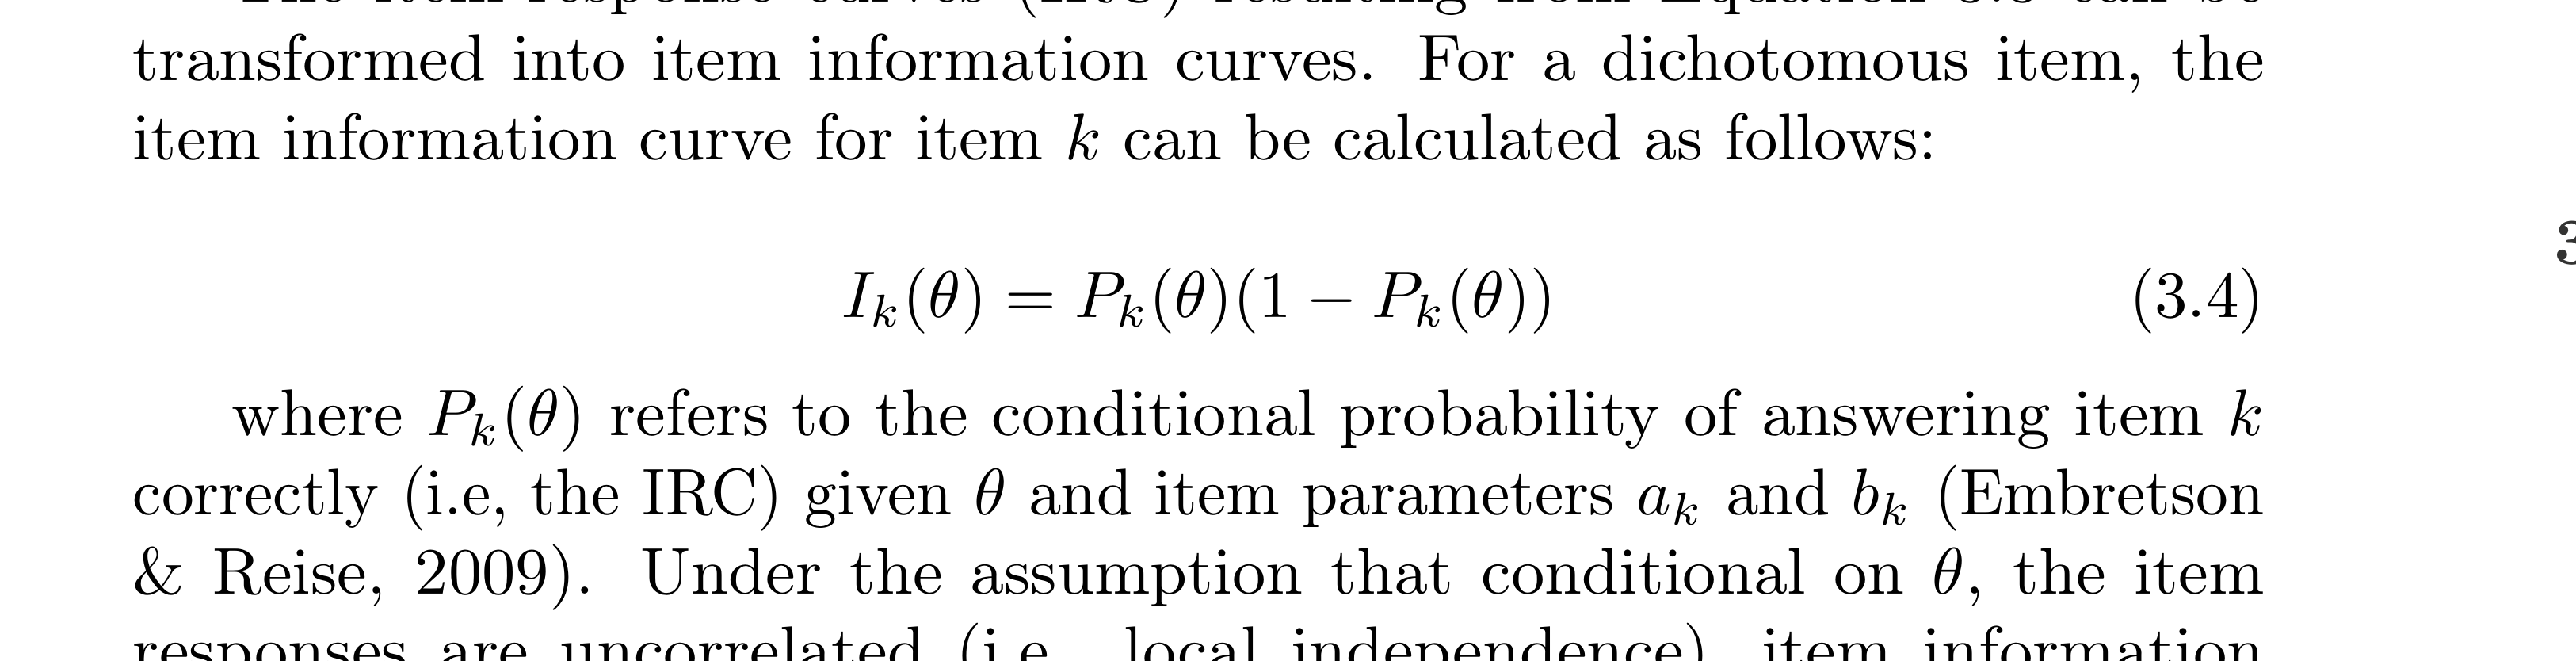
\includegraphics[width=.92\textwidth]{../evidence/eq3-information.png}\\[1em]
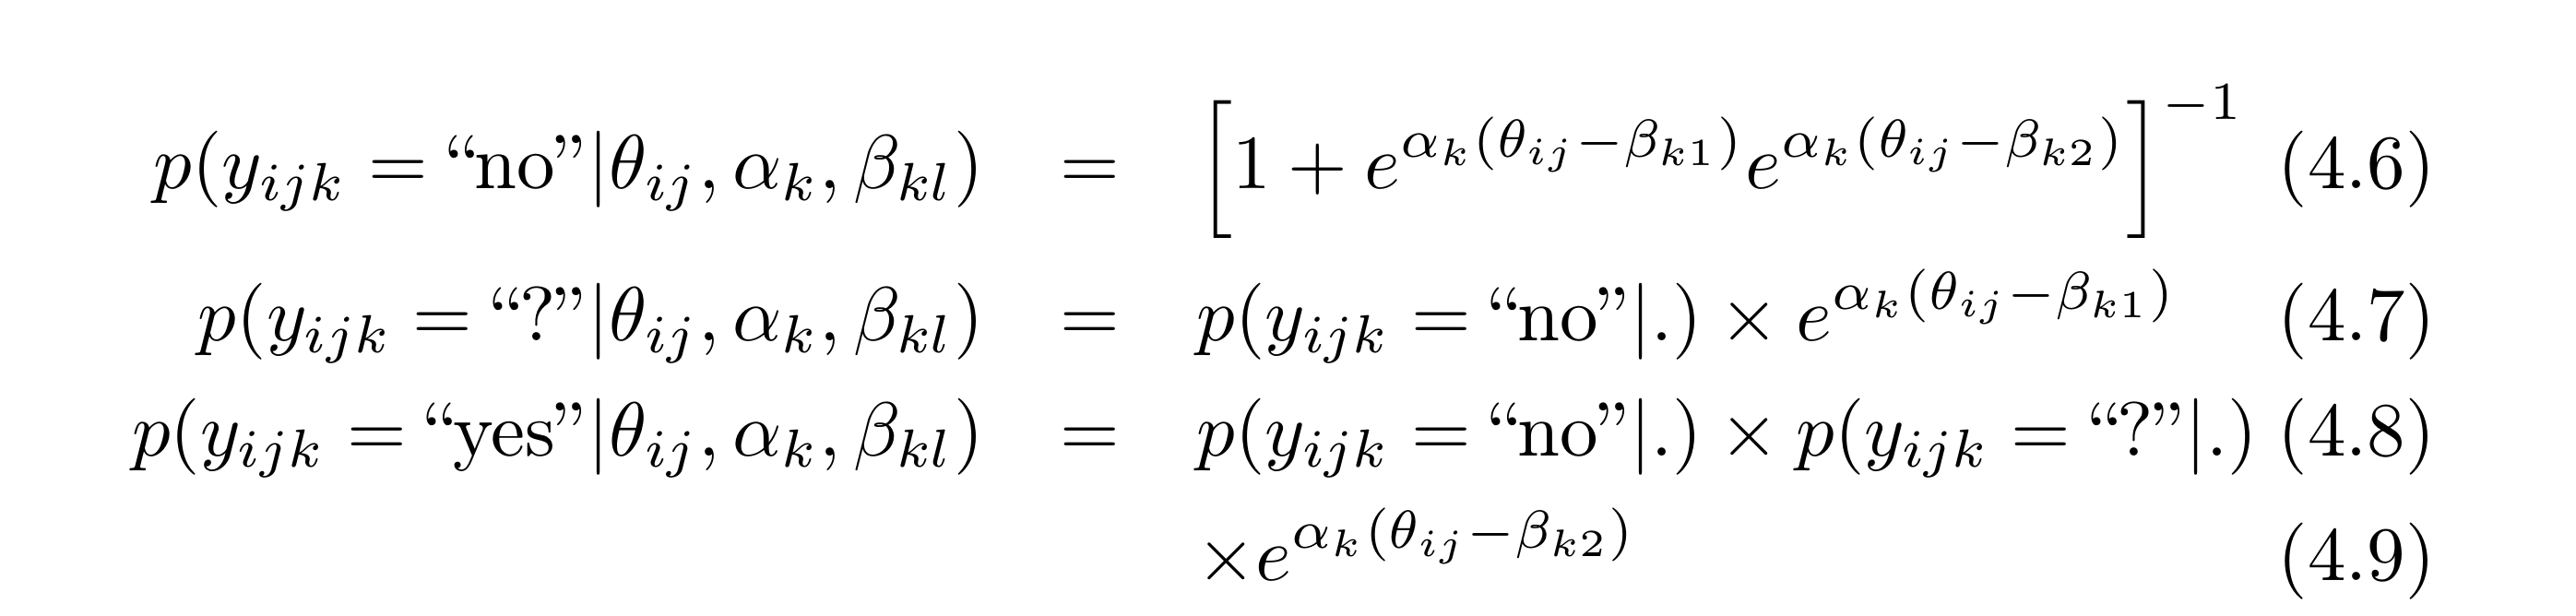
\includegraphics[width=.92\textwidth]{../evidence/eq4-probabilities.png}
\caption{Schwabe (2016), printed Equation 3.4 and Equations 4.6--4.9. Literal-expression checks do not establish which expressions the empirical analysis used.}
\end{figure}
\begin{figure}[p]\centering
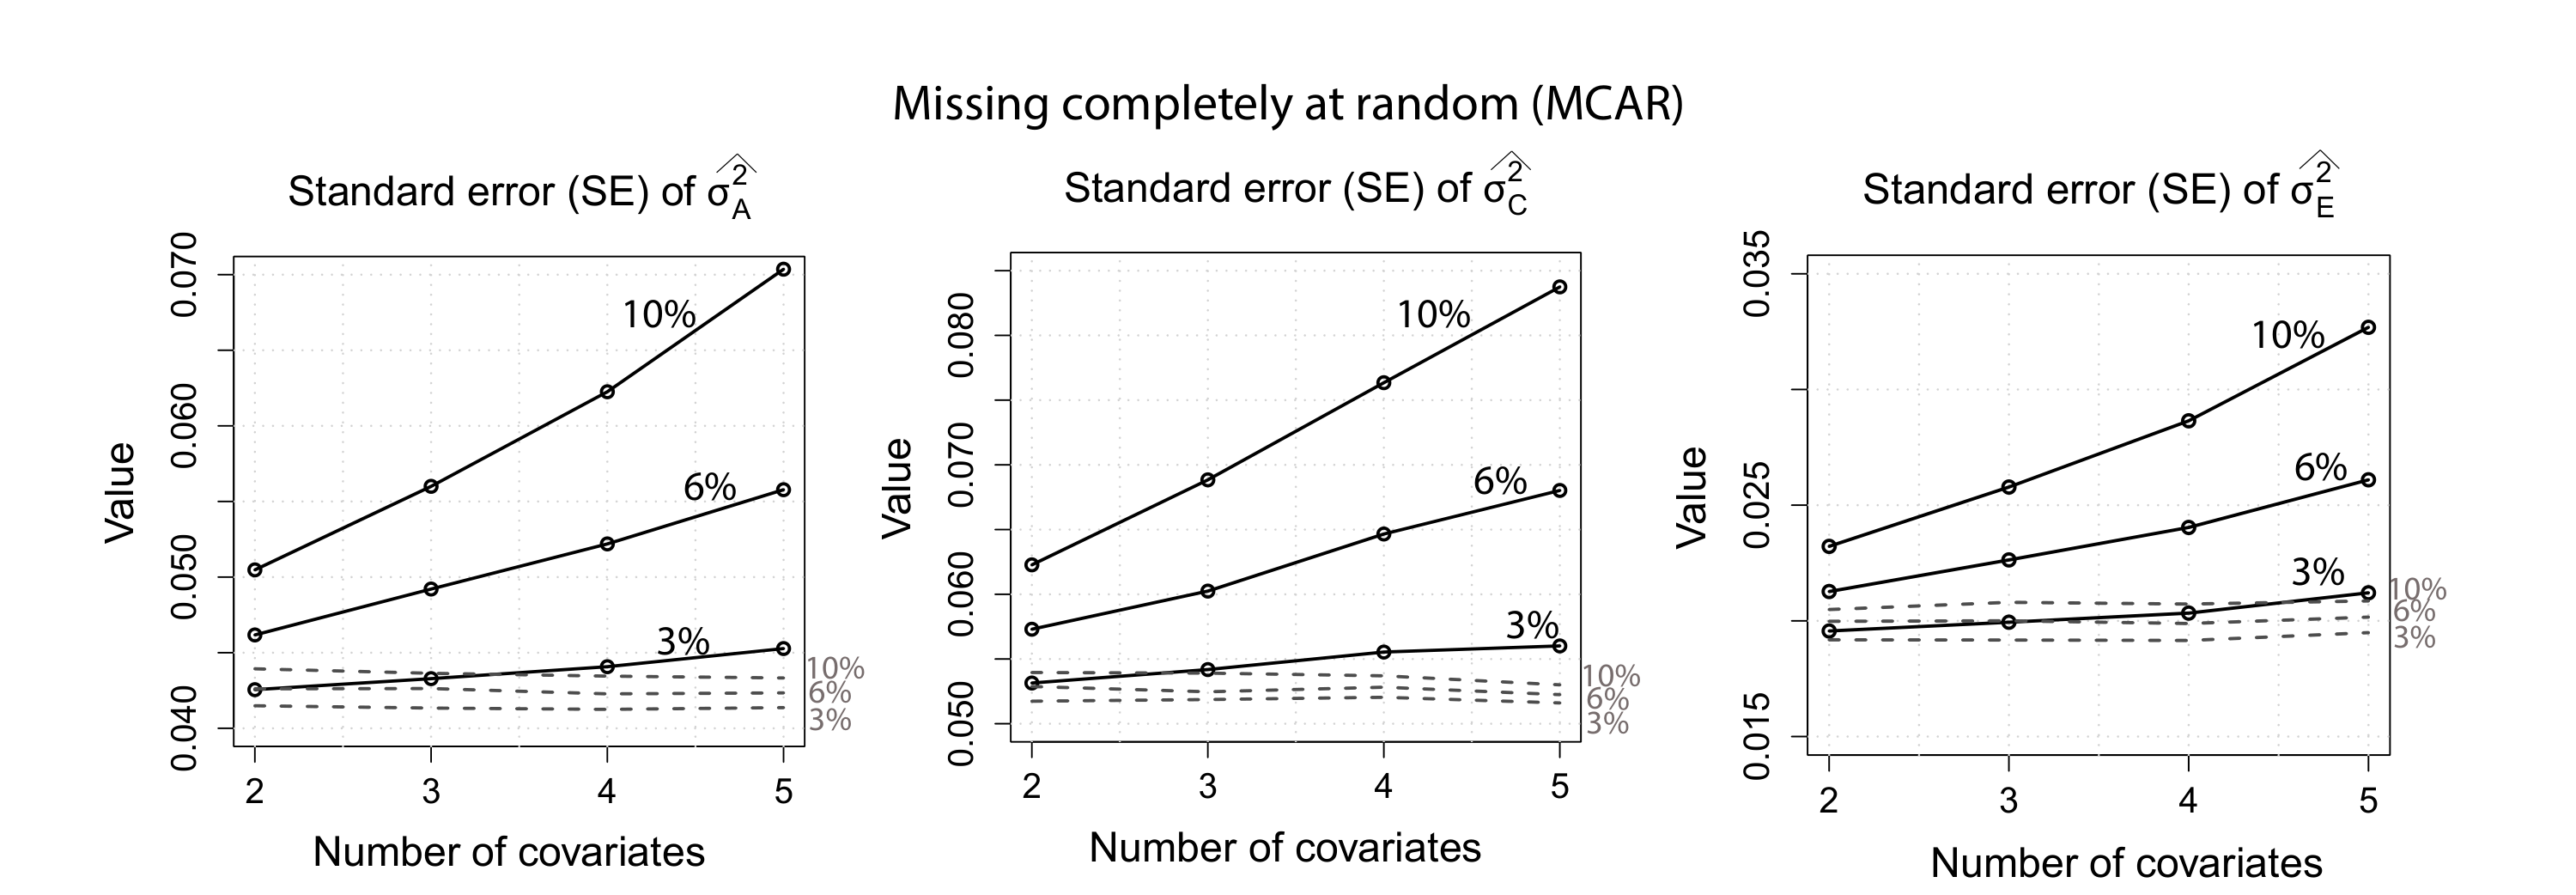
\includegraphics[width=.94\textwidth,height=.74\textheight,keepaspectratio]{../evidence/fig6-3.png}
\caption{Schwabe (2016), Figure 6.3, printed page 93. The source labels variance-component standard errors; reconstruction of path standard errors remains a distinct, exploratory hypothesis.}
\end{figure}
\clearpage

\bibliographystyle{plainnat}
\bibliography{references}
\end{document}
